\section{Server Konfiguration}
\subsection{Screenshots}
\begin{minipage}[t]{\textwidth}
	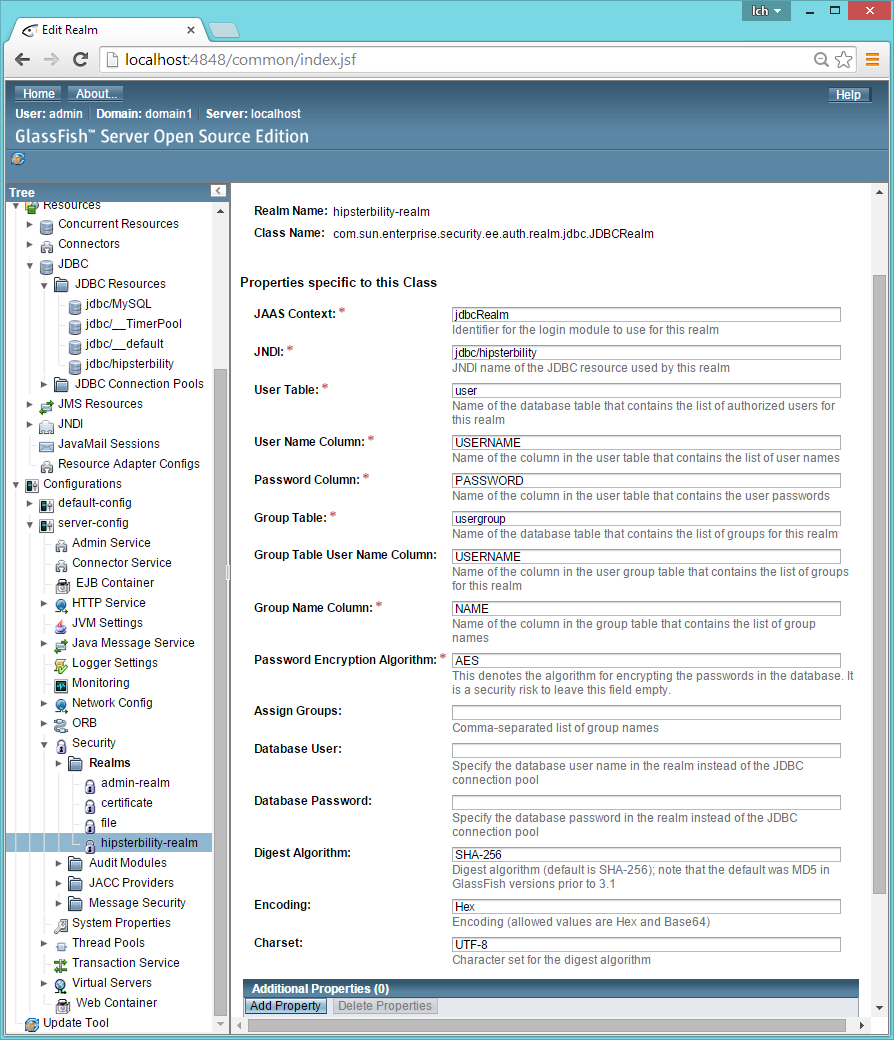
\includegraphics[width = \linewidth]{img/screenshot_realm.png}
	\captionof{figure}{Screenshot der Security-Realm Konfiguration des Glassfish Servers}
	\label{fig:realm_screenshot}
\end{minipage}

\newpage
\subsection{Glassfish Befehle}

\lstinputlisting[caption={Erstellen eines Glassfish Security Realms mit dem \enquote{asadmin} Werkzeug.},language=bash, firstline=2,label=lst:asadmin_create_realm]{../../UsabilityToolkit/HipsterbilityServer/src/main/scripts/glassfish-create.txt}


\subsection{Konfigurationsdateien}

\lstinputlisting[caption={persistence.xml für die Datenbankverbindung.},language=XML, label=lst:persistence_xml]{../../UsabilityToolkit/HipsterbilityServer/src/main/resources/META-INF/persistence.xml}


\lstinputlisting[caption={glassfish-resources.xml zum Erzeugen eines JDBC Resource-Pools und einer JDBC Ressource},language=XML,label=lst:glassfish-resources_xml]{../../UsabilityToolkit/HipsterbilityServer/src/main/scripts/glassfish-resources.xml}
